\documentclass[12pt]{article}
\usepackage[utf8]{inputenc}
\usepackage[T1]{fontenc}
\usepackage{fancyhdr} % Paquete para encabezados y pies de página
\usepackage{lipsum}
\usepackage{graphicx}   % Para texto de ejemplo (puedes omitirlo)
\usepackage{booktabs}
\usepackage{fontenc}
\usepackage{wrapfig}   % Para el entorno wrapfigure
\usepackage{caption}
\usepackage{multirow}  % Paquete para celdas que ocupan varias filas
\usepackage{colortbl}
\usepackage{color}

\usepackage{subcaption}
\usepackage{xcolor}
\usepackage{fourier}  % Incluye Utopia
%\usepackage{XCharter}      % Fuente serif XCharter
\usepackage{tgpagella}     % Fuente serif elegante TeX Gyre Pagella
\usepackage{tgheros}       % Fuente sans-serif TeX Gyre Heros (basada en Helvetica)
\usepackage{inconsolata}   % Fuente monoespaciada Inconsolata
%\usepackage[spanish]{babel}

\usepackage{lmodern}
\usepackage{libertinus}
% Configuración de encabezados y pies
\pagestyle{fancy}
\fancyhf{} % Limpia los encabezados y pies
\fancyhead[L]{UNAM - Escuela Nacional de Ciencias de la Tierra} % Encabezado izquierdo
\fancyhead[R]{Proyecto de Tesis}          % Encabezado derecho
\fancyfoot[C]{Página \thepage}            % Pie de página centrado

\begin{document}

% Crear la portada manualmente
\begin{titlepage}
    \begin{center}
        \vspace*{2cm} % Espacio vertical inicial
        {\Huge\bfseries Temas avanzados}\\[1cm]
        {\Large Autor: Nombre del Estudiante}\\[0.5cm]
        {\large Facultad de Ciencias, UNAM}\\[1cm]
        {\large \today}
    \end{center}
    \vfill % Espacio flexible para alinear verticalmente
    \begin{center}
        {\small Documento académico para el curso de Física del Clima}
    \end{center}
\end{titlepage}

Las figuras también se pueden mostrar en subpaneles, aunque esto se pueda hacer desde el programa original donde se generan las figuras. Por ejemplo, en Python esto se hace fácilmente con subplot. 

\begin{figure}
     \centering
     \begin{subfigure}[b]{0.3\textwidth}
         \centering
         
\includegraphics[width=\textwidth]{dog1.jpg}
         \caption{Perrito 1.}
         \label{fig:a}
     \end{subfigure}
     \hfill
     \begin{subfigure}[b]{0.3\textwidth}
         \centering
         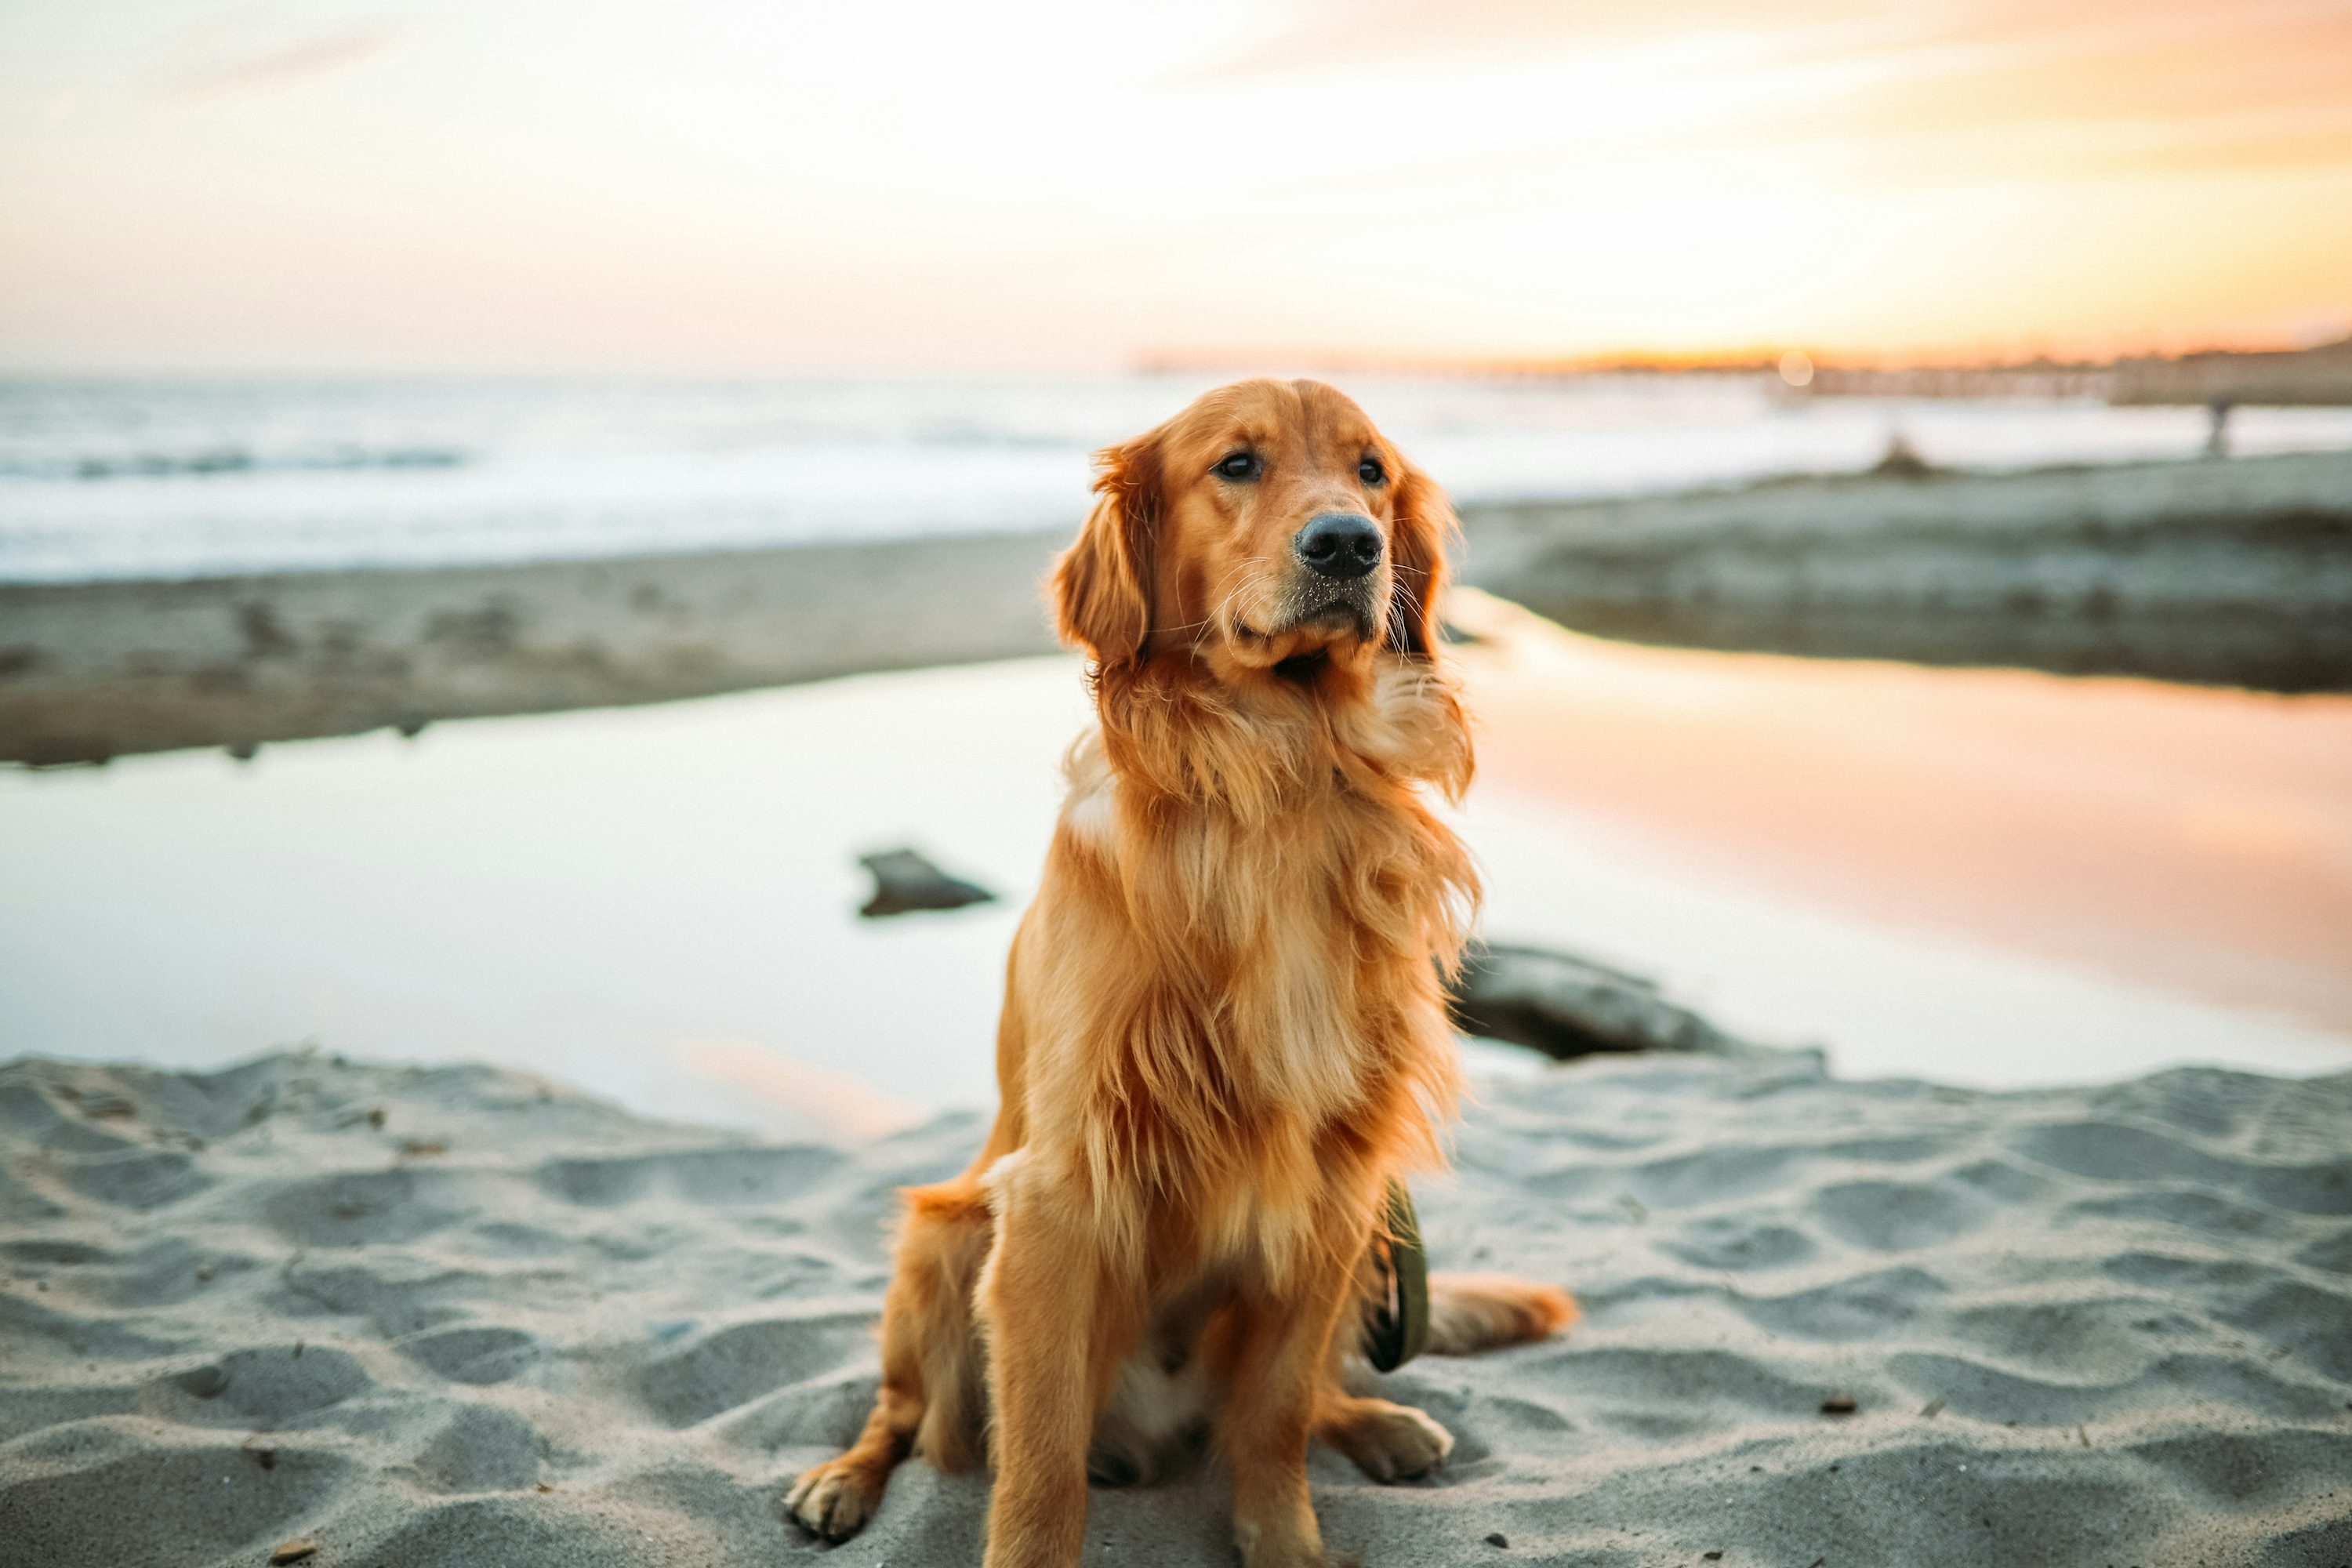
\includegraphics[width=\textwidth]{dog2.jpeg}
         \caption{Perrito 2}
         \label{fig:b}
     \end{subfigure}
     \hfill
     \begin{subfigure}[b]{0.3\textwidth}
         \centering
         
\includegraphics[width=\textwidth]{Leonardo.jpg}
         \caption{Nubes}
         \label{fig:c}
     \end{subfigure}
        \caption{3 figuras horizontales}
        \label{fig:three graphs}
\end{figure}

Para referenciar este entorno con 3 figuras, podemos llamar a la Figura principal, como Fig. \ref{fig:three graphs} o hacer referencia espec\'ifica a una figura, como la Fig. \ref{fig:c}.

\section{El entorno \texttt{wrapfigure}}

El entorno \texttt{wrapfigure} es útil para insertar figuras rodeadas de texto, permitiendo que el flujo no se interrumpa completamente. Este entorno es particularmente eficiente en documentos donde se busca aprovechar mejor el espacio.

El entorno \texttt{wrapfigure} tiene varios elementos importantes:
\begin{itemize}
    \item \textbf{Posición:} El primer argumento define la alineación. Puede ser \texttt{r} (derecha), \texttt{l} (izquierda) o \texttt{c} (centrado).
    \item \textbf{Ancho:} El segundo argumento especifica el ancho de la figura en relación al ancho del texto, por ejemplo, \texttt{0.4\textbackslash textwidth}.
    \item \textbf{\texttt{\textbackslash includegraphics}:} Este comando inserta la imagen. Puedes ajustar el tamaño con \texttt{width}, \texttt{height} u otros parámetros.
    \item \textbf{\texttt{\textbackslash caption}:} Agrega un pie de figura explicativo.
    \item \textbf{\texttt{\textbackslash label}:} Permite referenciar la figura en otras partes del texto usando \texttt{\textbackslash ref}.
\end{itemize}

\lipsum[3]

\begin{wrapfigure}{l}{0.35\textwidth}  % Figura alineada a la izquierda
    \centering
    
\includegraphics[width=0.3\textwidth]{dog1}
    \caption{Perrito 1 con el texto.}
    \label{fig:wrapfigure}
\end{wrapfigure}

\lipsum[4]

\section{Tabla Compleja}

El siguiente ejemplo muestra una tabla con múltiples encabezados y combinaciones de celdas:

\begin{table}[h]
    \centering
    \begin{tabular}{|l|c|c|c|}
        \hline
        \multirow{2}{*}{\textbf{Variable}} & \multicolumn{3}{c|}{\textbf{Frecuencia de Muestreo}} \\ \cline{2-4}
        & Diario & Mensual & Anual \\ \hline
        Temperatura & 24.5°C & 23.1°C & 22.9°C \\ \hline
        Precipitación & 5.4 mm & 120 mm & 1450 mm \\ \hline
        Humedad Relativa & 65\% & 60\% & 58\% \\ \hline
    \end{tabular}
    \caption{Datos de variables atmosféricas con distintas frecuencias de muestreo.}
    \label{tab:variables}
\end{table}

Como se muestra en la Tabla \ref{tab:variables}, las variables cambian según la frecuencia de muestreo.







\section{Colores}

{\color{blue}\lipsum[4]}

{\color{red}\lipsum[4]}


section{Ejemplo de Cambio de Fuentes}

En este ejemplo, mostramos cómo utilizar diferentes fuentes en el mismo documento. Para cada párrafo, aplicamos una fuente distinta.

\subsection*{1. Fuente: TeX Gyre Pagella (serif elegante)}
% Fuente predeterminada del documento
{ \fontfamily{XCharter-TLF}\selectfont
\lipsum[1]
}

\subsection*{2. Párrafo con Latin Modern Roman}
% Cambio a Latin Modern temporalmente
{\fontfamily{lmr}\selectfont
\lipsum[2]
}

\subsection*{3. Fuente: TeX Gyre Heros (sans-serif moderno)}
% Cambio a sans-serif temporalmente
{\sffamily 
\lipsum[2]
}

\subsection*{4. Fuente: Inconsolata (monoespaciado para código)}
% Cambio a fuente monoespaciada
{\ttfamily 
\lipsum[3]
}

\vspace{2mm}

Este ejemplo utiliza tres fuentes recomendadas para documentos académicos:

\color{teal}

{\fontfamily{put}\selectfont   Aquí el texto comienza con la fuente \textbf{Utopia}, que es una opción moderna y legible para trabajos académicos. }

{\fontfamily{qpl}\selectfont Luego cambiamos a \textbf{TeX Gyre Pagella}, una fuente serif elegante y ligeramente más formal. \lipsum[1]} 

 {\fontfamily{lmr}\selectfont O la clásica Latin Modern. \lipsum[1] } 

{\fontfamily{LibertineT}\selectfont Aquí el texto está en Libertinus Serif.}


Finalmente, {\sffamily \textbf{Libertinus Sans}} es una fuente sans-serif ideal para presentar secciones más ligeras o encabezados.


\end{document}
